\documentclass[a4paper,12pt]{article}
%\usepackage[utf8x]{inputenc}
\usepackage{amssymb}
\usepackage{amsfonts}
\usepackage{mathrsfs}
\usepackage{amsmath}
\usepackage{amsthm}
\usepackage[margin=3cm]{geometry}
\usepackage{times}
\usepackage{graphicx}
%\usepackage{enumitem}
\usepackage{fancyhdr}
\usepackage{hyperref}
\usepackage{setspace}
\usepackage{subcaption}
\usepackage{mathtools}

\pagestyle{fancy}
\fancyhf{}
\lhead{Thomas J. Delaney}
\rhead{Forecasting Methods}
\cfoot{\thepage}

\newtheorem{theorem}{Theorem}
\newtheorem{proposition}{Proposition}[section]
\newtheorem{lemma}{Lemma}[section]
\newtheorem{corollary}{Corollary}[section]
\theoremstyle{definition}
\newtheorem{definition}{Definition}[section]

\newcommand{\boldnabla}{\mbox{\boldmath$\nabla$}} % to be used in mathmode
\newcommand{\cbar}{\overline{\mathbb{C}}}% to be used in mathmode
\newcommand{\diff}[2]{\frac{d #1}{d #2}}% to be used in mathmode
\newcommand{\difff}[2]{\frac{d^2 #1}{d #2^2}}% to be used in mathmode
\newcommand{\pdiff}[2]{\frac{\partial #1}{\partial #2}} % to be used in mathmode
\newcommand{\pdifff}[2]{\frac{\partial^2 #1}{\partial #2^2}}% to be used in mathmode
\newcommand{\upperth}{$^{\mbox{\footnotesize{th}}}$}%to be used in text mode
\newcommand{\vect}[1]{\mathbf{#1}}% to be used in mathmode
\newcommand{\curl}[1]{\boldnabla \times \vect{#1}} % to be used in mathmode
\newcommand{\divr}[1]{\boldnabla \cdot \vect{#1}} %to be used in mathmode
\newcommand{\modu}[1]{\left| #1 \right|} %to be used in mathmode
\newcommand{\brak}[1]{\left( #1 \right)} % to be used in mathmode
\newcommand{\comm}[2]{\left[ #1 , #2 \right]} %to be used in mathmode
\newcommand{\dop}{\vect{d}} %to be used in mathmode
\newcommand{\cov}{\text{cov}} %to be used in mathmode
\newcommand{\var}{\text{var}} %to be used in mathmode
\newcommand{\mb}{\mathbf} %to be used in mathmode
\newcommand{\bs}{\boldsymbol} %to be used in mathmode
% Title Page
\title{Forecasting Methods: An Overview}
\date{}
\author{Thomas J. Delaney}

\begin{document}

\maketitle

\tableofcontents

\newpage

\section{Introduction}
An overview of forecasting methods, from the simplest to the most up to date.

\subsection{What is Forecasting?}
A \textit{time series} is list of measurements or recordings ordered by the time at which those measurements were taken, or those recordings were made. \textit{Forecasting} is the act of predicting the future value of a quantity (usually a time series) with some measure of confidence. Every forecasting method consists of constructing a model of the series, and basing a mean prediction and prediction interval on that model. 

\subsubsection{Example: The Na\"{i}ve Method}\label{sec:naive_method}
For example, one of the simplest forecasting methods is the \textit{na\"{i}ve} method. This consists of forecasting that the next value of the time series will be sampled from a normal distribution (aka. Gaussian distribution) with mean equal to the latest value of the time series, and standard deviation equal to the standard deviation of the one step changes in the time series. Using this model, the forecasted value for the time series is same as the latest value, and the prediction intervals are calculated using the z-distribution.

More formally, if $y_1, \dots, y_T \in \mathbb{R}$ is a time series and $d_1, \dots, d_{T-1}$ are the one step differences of that series, then according to the na\"{i}ve model 
\begin{equation}\label{eq:naive_method}
	\hat{y}_{T+1 | 1, \dots, T} \sim \mathcal{N}(y_T, \sigma^2)
\end{equation}
where $\sigma^2$ is the variance of $d_1, \dots, d_{T-1}$. As for prediction intervals, since the z-statistic for $95\%$ is $1.96$, the $95\%$ prediction interval for $\hat{y}_{T+1 | 1, \dots, T}$ is $\pm1.96\sigma$.

\section{Residuals, Normality\& Prediction Intervals}
In a forecasting context, a residual is the difference between a given time series value and the one step forecast for that value, $e_t = y_t - \hat{y}_{t | 1, \dots , t-1}$. Given some forecasting model,these residuals are usually used to determine the amount of noise in the model and calculate the prediction intervals. It should be noted that since the z-distribution is always used to calculate the prediction intervals, the residuals of the model must be distributed normally. Otherwise the intervals will be inaccurate. Effectively, the noise in any model is always modelled as white noise,
\begin{equation}\label{eq:white_noise}
	\epsilon_t \sim \mathcal{N}(0, \sigma^2)
\end{equation}
where $\sigma^2$ is the variance of the residuals.

In the example given in section \ref{sec:naive_method}, since the model forecasts the next value in the series to be the same as the last, the residuals are the one step differences of the series. Another way of formulating the model given by equation \ref{eq:naive_method} is
\begin{align}
	\hat{y}_{T+1 | 1, \dots, T} = y_T + \epsilon_t
\end{align}

\section{Random Walks, Transformations, \& Stationarity}

\subsection{Random Walk Forecasting}
% consider putting random walk in with ETS and ARIMA altogether

Random walk is another simple method for forecasting in which the one step change in the time series is modelled. The simplest version models the one step change as a normal distribution with zero mean. This is the same as the na\"{i}ve model in section \ref{sec:naive_method}. The model can be expanded to include a \textit{drift} term so that
\begin{align}
	\hat{y}_{T+1|1, \dots, T} - y_T \sim \mathcal{N}(c, \sigma^2)
\end{align}
where $c \in \mathbb{R}$ and $\sigma^2$ is the variance of the residuals. If $c > 0$ then  the series will show an upward linear trend, and if $c<0$ the series will show a downward linear trend. Another way of formulating this model is
\begin{align}
	\hat{y}_{T+1|1, \dots, T} = y_T + c + \epsilon_t
\end{align}
where $\epsilon_t$ is defined by equation \ref{eq:white_noise}, as usual.

\subsection{Seasonally Adjusted Random Walk}
A random walk model can be used to forecast time series with a seasonal pattern. If there are $m$ seasons, that is, if the seasonality has a period of $m$ time-steps then the forecasted value will be based on the value of the previous season, rather than the previous time step
\begin{align}
	\hat{y}_{T+1|1, \dots, T}  - y_{T+1-m} \sim \mathcal{N}(c,\sigma^2) \hspace{5mm} \text{or} \hspace{5mm} \hat{y}_{T+1|1, \dots, T} =  y_{T+1-m} + c + \epsilon_t
\end{align}

These random walk models are sometimes called \textit{difference models} because the forecast is based upon the difference between previous values of the series, with some lag applied. 

\subsection{Transformations for Stationarity}
A stationary time series is one whose properties do not depend on the time at which the series is observed, or more precisely if $\{y_t\}$ is a stationary time series, then for all $s$, the distribution of $(y_t, \dots ,y_{t+s})$ does not depend on $t$. A white noise time series (equation \ref{eq:white_noise}) is an example of a stationary series. The aim of most simple forecasting models is to capture all the variance of a time series, except for some additional or multiplicative white noise. This means that the model will often consist of applying transformations to the time series until the series is stationary. 

For example, the na\"{i}ve model captures the amplitude or \textit{level} of the time series by taking the one step difference, leaving only white noise thereafter. A seasonal random walk model with a non-zero drift parameter will capture the amplitude of the time series at each season, and the overall trend of the time series, leaving only white noise thereafter. Some non-linear trends can be captured using a Box-Cox transformation. 
\begin{align}
	y_{t, (\lambda)} = \begin{cases}
					\frac{y_t^\lambda - 1}{\lambda} &\quad \text{if } \lambda \neq 0 \\
					\ln(y_t) &\quad \text{if } \lambda = 0 
				\end{cases}
\end{align}

If multiplicative noise is observed in the time series, it's common to apply a log transformation in order to the make the noise additive, or a Box-Cox transformation with $\lambda = 0$. In the case where the time series may take values less than or equal to zero, the Yeo-Johnson transforamtion is used to capture non-linearity,
\begin{align}
	y_{t, (\lambda)} = \begin{cases}
					\frac{(y_t + 1)^\lambda - 1}{\lambda} &\quad \text{if } \lambda \neq 0, y_t \geq 0 \\
					\ln(y_t + 1) &\quad \text{if } \lambda = 0, y_t \geq 0 \\
					-\frac{[(-y_t + 1)^{2-\lambda}-1]}{2-\lambda} &\quad \text{if } \lambda \neq 2, y_t < 0 \\
					-\ln(-y_t + 1) &\quad \text{if } \lambda = 2, y_t < 0
				\end{cases}
\end{align}
where $0 \leq \lambda \leq 2$. 

\section{ARIMA}
\subsection{Auto-regression models}
Auto-regression models are exactly what they sound like. They use a linear combination of some of the previous elements of the time series to forecast the upcoming values. The number of values used is determined by the \textit{degree}, $p$. A degree-$p$ auto-regressive model can be written as
\begin{equation}\label{eq:ar_model}
	\hat{y}_{T|1, \dots, T-1} = c + \phi_1 y_{T-1} + \phi_2 y_{T-2} + \cdots + \phi_p y_{T-p} + \epsilon_t
\end{equation}
where $\epsilon_t$ is the usual white noise. A model of this kind of often denoted as $AR(p)$.

Notice that the $c$ term can capture a linear trend in the series. An $AR(1)$ model with $\phi_1 = 1$ is equivalent to a random walk with a trend.

In order for the modelled series to be stationary some restrictions must be applied to the parameter values. Specifically, for an $AR(p)$ model the roots of the polynomial
\begin{align}
	z^p - \sum_{i=1}^{p} \phi_{i}z^{p-i}
\end{align}
must lie within the complex unit circle, $\modu{z_i} < 1$. Practically, this amounts to having $\modu{\phi_1}<1$ for an $AR(1)$ model, and $\modu{\phi_2}<1$, and $\phi_1 + \phi_2 <1$ for $AR(2)$.

The most suitable order for an $AR(p)$ model can be determined by looking at the $ACF$ and $PACF$ of the time series. The lag beyond which the $PACF$ appears to be zero is the most suitable order.

\subsection{Moving-average models}
\textit{Moving average model} is a poor name for this model, but it is the conventional name. A better name would be \textit{residual-regression model} because the forecast is a linear combination of past residuals. A moving average model or order q can be written as
\begin{equation}
	\hat{y}_{T|1, \dots, T-1} = c + \epsilon_t + \theta_1 \epsilon_{t-1} + \cdots + \theta_q \epsilon_{t-q}
\end{equation}
where $\epsilon_t$ is the usual white noise. This type of model is usually denoted $MA(q)$.

If a moving average model can be expressed as an infinite degree AR model, the moving average model is called \textit{invertible}. 

\subsection{ARIMA models}
Auto-regression, difference, and moving average models can be combined. A combination of an $AR(p)$, $d$-step difference, and $MA(q)$ model is denoted $ARIMA(p,d,q)$. $ARIMA$ stands for \textit{Auto-regressive integrated moving average}. To construct an $ARIMA(p,d,q)$ model, first $\{y_t\}$ is transformed to $\{ y_t^{\prime} \}$ by taking the $d$-step difference, then
\begin{equation}
	\hat{y}_{T|1,\dots,T-1}^{\prime} = c + \phi_1 y_{T-1}^{\prime} + \cdots + \phi_{p} y_{T-p}^{\prime} + \epsilon_t + \theta_{1} \epsilon_{t-1} + \cdots + \theta_{q} \epsilon_{t-q}
\end{equation}
The degree of the $AR$ and the order of the $MA$ that should be used can be determined from a combination of the $ACF$ and the $PACF$. The number of differences to use is generally two or fewer. This can be determined by examining the long term trend of the data.

\subsubsection{Seasonal ARIMA models}
In order to capture seasonal behaviour in the time series, a \textit{seasonal ARIMA} model can be used. This is an additional $ARIMA$ model where all the lags are the length of one season. The length of a season will have to be found by inspection. The additional seasonal $ARIMA$ terms are  just multiplied by the standard $ARIMA$ terms.

\section{Error, Trend, Smoothing models (ETS models)}
\subsection{Simple Exponential Smoothing}
If a time series has no clear trend, seasonality, or cycle but appears to vary around some fixed amplitude, simple exponential smoothing might be a suitable forecasting method. In simple exponential smoothing, the forecast is an weighted sum of the series's previous values where the weights decrease exponentially going backwards in time.
\begin{align}
	\hat{y}_{T+1 | T,\dots,1} = \alpha y_T + \alpha(1-\alpha)y_{T-1} + \alpha(1-\alpha)^2y_{T-2} + \cdots
\end{align}
where $0 \leq \alpha \leq 1$ is the smoothing parameter. If $\alpha$ is close to $0$, a large weight will be given to values in the distant past. If $\alpha$ is close to $1$, more recent values will get a larger weight, which usually makes sense. In the extreme case where $\alpha = 1$ the forecast will be same as the mean forecast of the na\"{i}ve method.

Basically just decompose the time series into level, trend, and seasonal components. The seasonal component can be multiplicative or additive. Simple exponential smooting is usually written in one of two ways. The weighted average form is
\begin{align}
	\hat{y}_{T+1|T,\dots,1} = \alpha y_T + \left(  1 - \alpha \right)\hat{y}_{T|T-1,\dots,1}
\end{align}
Note that the second term on the right hand side is a forecasted value, and therefore accounts for all the values of $\left\{ y_t \right\}$ where $t < T$.

The component form is
\begin{align}
	\hat{y}_{T+1|T,\dots,1} &= \ell_T \label{eq:ses_forecast}\\
	\ell_T &= \alpha y_T	+ (1 - \alpha)\ell_{T-1} \label{eq:ses_smoothing}
\end{align}
Equation \ref{eq:ses_forecast} is called the \textit{forecast equation}, and equation \ref{eq:ses_smoothing} is called the \textit{smoothing equation} or the \textit{level equation}. The practicality of the component form will be clearer when trend and seasonal components are introduced.

When implementing exponential smoothing, the $\alpha$ and $\ell_0$ are parameters that must be fitted. The usual way of fitting the parameters is by minimising the sum of the squared errors between the timer series and the fitted values,
\begin{align}
	SSE =  \sum_{t=1}^T\left( y_t - \hat{y}_{t|t-1} \right)^2
\end{align}
This is a non-linear optimisation problem for which there is no analytical solution, so an optimisation algorithm must be used. Usually this will be built into whatever programming language is used for implementation.

\subsection{Holt's Linear Trend Method}
Simple exponential smooting can be extended to time series with a trend by including another smoothing equation.
\begin{align}
	\hat{y}_{T+h|T,\dots,1} &= \ell_T + hb_T \label{eq:holt_forecast}\\
	\ell_T &= \alpha y_T + (1 - \alpha)\left(\ell_{T-1} + b_{T-1}\right) \label{eq:holt_level} \\
	b_T &= \beta^*\left( \ell_t - \ell_{t-1} \right) + (1 - \beta^*)b_{T-1} \label{eq:holt_trend}
\end{align}
where $0 \leq \beta^* \leq 1$. Equations \ref{eq:holt_forecast} and \ref{eq:holt_level} are the forecast and level equations as before. Equation \ref{eq:holt_trend} is called the \textit{trend equation}. The trend for a given timestep is a weighted sum of the change in the level beteen this time-step and the last time-step, and the previous trend. The level equation is influenced by the trend of the previous step. The forecast equation has a trending component.

Holt's linear method will give a forecast that is linear in the forecast horizon. A slightly better approach is to used the damped version.
\begin{align}
	\hat{y}_{T+h|T,\dots,1} &= \ell_T + \left( \phi + \phi^2 + \cdots + \phi^h \right)b_T \label{eq:holt_forecast}\\
	\ell_T &= \alpha y_T	+ (1 - \alpha)\left(\ell_{T-1} + \phi b_{T-1}\right) \label{eq:holt_level} \\
	b_T &= \beta^*\left( \ell_t - \ell_{t-1} \right) + (1 - \beta^*)\phi b_{T-1} \label{eq:holt_trend}
\end{align}
where $0 < \phi < 1$ is the damping coefficient. This method gives a forecast which is linear initially but approaches 
\begin{align}
	\ell_T + \frac{\phi}{1-\phi} b_T \quad \text{ as } h \rightarrow \infty
\end{align}

\subsection{Holt-Winter's Seasonal Method}\label{sec:hw_seasonal}
Introducing another smoothing equation can account for seasonal variations. The seasonal component can be additive or multiplicative. The additive version is,
\begin{align}
	\hat{y}_{T+h|T,\dots,1} &= \ell_T + hb_T + s_{T+h-m(k+1)} \label{eq:hw_forecast}\\
	\ell_T &= \alpha (y_T - s_{T-m}) + (1 - \alpha)\left(\ell_{T-1} + b_{T-1}\right) \label{eq:hw_level} \\
	b_T &= \beta^*\left( \ell_t - \ell_{t-1} \right) + (1 - \beta^*)b_{T-1} \label{eq:hw_trend} \\
	s_T &= \gamma \left( y_T - \ell_{T-1} - b_{T-1} \right) + \left( 1 - \gamma \right)s_{t-m} \label{eq:hw_seasonal}
\end{align}
where $k$ is the integer part of $(h-1)/m$, i.e. the number of seasons in the forecast horizon, and $0 \leq \gamma \leq 1 - \alpha$. Equation \ref{eq:hw_seasonal} is called the seasonal equation. This equation shows that the seasonal component is the weighted average of the seasonal index from this year $(y_t - l_{t-1} - b_{t-1})$ and last year $s_{t-m}$. The quantity $y_t - s_t$ is the \textit{deseasonalised series}.

The multiplicative version is very similar
\begin{align}
	\hat{y}_{T+h|T,\dots,1} &= (\ell_T + hb_T)s_{T+h-m(k+1)} \label{eq:hw_forecast}\\
	\ell_T &= \alpha \frac{y_T}{ s_{T-m}} + (1 - \alpha)\left(\ell_{T-1} + b_{T-1}\right) \label{eq:hw_level} \\
	b_T &= \beta^*\left( \ell_t - \ell_{t-1} \right) + (1 - \beta^*)b_{T-1} \label{eq:hw_trend} \\
	s_T &= \gamma \frac{y_T}{\ell_{T-1} + b_{T-1}} + \left( 1 - \gamma \right)s_{t-m} \label{eq:hw_seasonal}
\end{align}
with the same resitrictions on the parameters. In this case, the deseasonalised series is $y_t/s_t$.

It's also possible to dampen the Holt-Winter's seasonal method in the same way as Holt's Linear method by introducing a damping parameter $\phi$.

\subsection{State Space Models}
These expoential smoothing models are lacking an estimate for their error. When an error estimation is added to make these models complete, they are usually called \textit{state space} models.

Equations \ref{eq:ses_forecast} and \ref{eq:ses_smoothing} can be re-written as
\begin{align}
	y_t &= \ell_{t-1} + \epsilon_t \label{eq:ss_measurement} \\
	\ell_t &= \ell_{t-1} + \alpha \epsilon_t \label{eq:ss_state}
\end{align}
where $\epsilon_t = y_t - \ell_{t-1}$, the $t$th residual. Equation \ref{eq:ss_measurement} is called the measurement equation and equation \ref{eq:ss_state} is called the state equation. 

Errors can also be multiplicative. If 
\begin{align}
	\epsilon_t = \frac{y_t - \hat{y}_{t|t-1,\dots,1}}{\hat{y}_{t|t-1,\dots,1}}
\end{align}
then the measurement and state equations become
\begin{align}
	y_t &= \ell_{t-1}(1 + \epsilon_t) \\
	\ell_t &= \ell_{t-1}(1 + \alpha \epsilon_t)
\end{align}
In both cases $\epsilon \sim \mathcal{N}(0, \sigma^2)$.

As an example Holt's linear method with additive errors is defined by 
\begin{align}
	y_t &= \ell_{t-1} + b_{t-1} + \epsilon_t \\
	\ell_t &= \ell_{t-1} + b_{t-1} + \alpha \epsilon_{t} \\
	b_t &= b_{t-1} + \beta \epsilon_t 
\end{align}
where $\epsilon \sim \mathcal{N}(0,\sigma^2)$, and $\beta = \alpha\beta^*$.

\subsection{ETS($\cdot,\cdot,\cdot$)}
State space models are often denoted by the method error, trend, and seasonality used. The type of error can be additive, $A$, or multiplicative $M$. The type of trend can be none $N$, additive $A$, and additive but dampened $A_d$. The type of seasonality can be none, additive, or multiplicative. There are 18 different types of state space model. They are all summarised in figure \ref{fig:ets_models}.

\begin{figure}[ht]
	\centering
	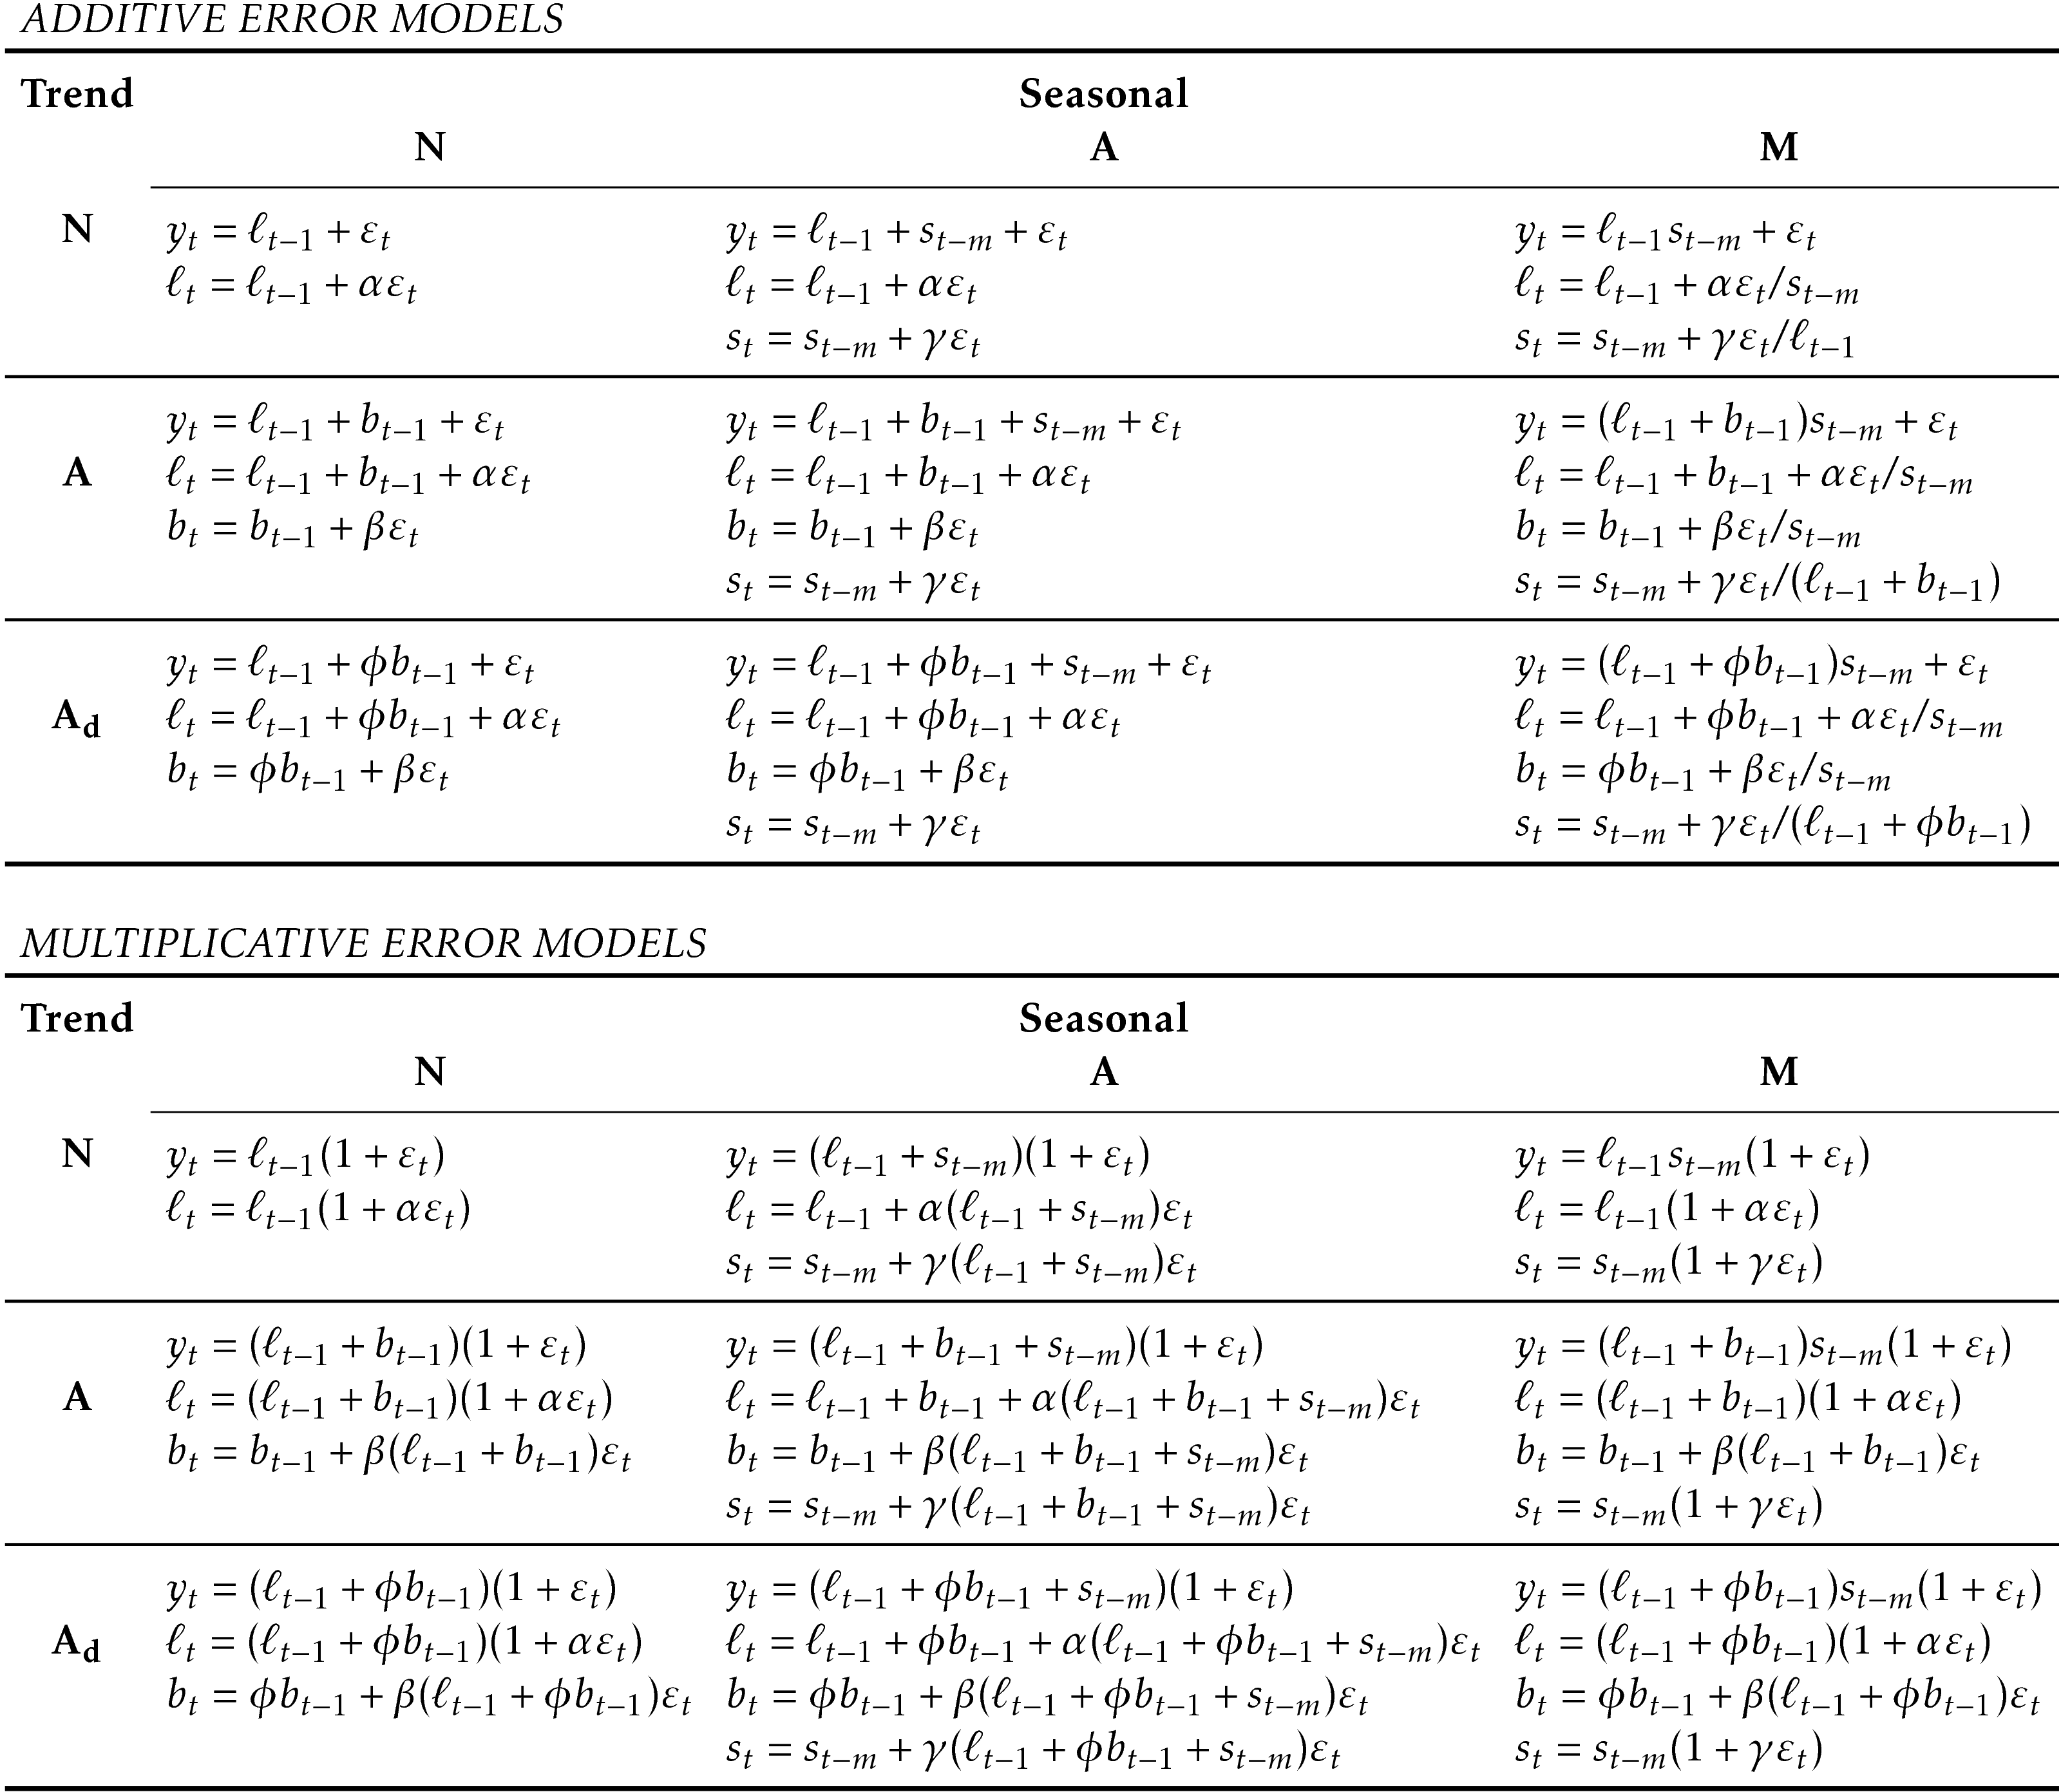
\includegraphics[width=\textwidth]{figures/ets_models.png}
	\caption{All possible ETS models. From \cite{fpp}.}
	\label{fig:ets_models}
\end{figure}

\section{Modelling the Volatility: ARCH, GARCH}
Until this section, all of the models mentioned in this document have noise with a constant variance. The models in this section are used for modelling the variance in the noise. ARCH stands for auto-regressive conditional heteroskedasticity. The `skedasticity' part of the heteroskedasticity comes from the Greek \textit{skedastikos}, meaning `able to disperse'. A \textit{homoskedastic} variable is dispersed by the same amount all the time, i.e. with constant variance, whereas a \textit{heteroskedastic} variable has a variance that changes over time. 

An ARCH model models the variance of the noise as an auto-regressive variable. If $\epsilon_t$ is the noise of the model, say
\begin{align}
	\epsilon_t = \sigma_t z_t
\end{align}
where $z_t \sim \mathcal{N}(0,1)$ is white noise, and 
\begin{align}
	\sigma^2_t = \alpha_0 + \sum_{i=1}^q \alpha_i \epsilon_{t-i}^2
\end{align}
is an $AR(q)$ model for the variance of the noise. When an $AR(q)$ model is used to model the volatility of a time series, the volatility at any given time step will be correlated with the previous steps. If the volatility is modelled using white noise, the volatility will be uncorrelated.

If an $ARMA(q,p)$ is used to model the volatility, this is called a generalised auto-regressive conditional heteroskedasticity model, or GARCH model. In this case
\begin{align}
	\sigma^2_t = \omega + \sum_{i=1}^q \alpha_i \epsilon_{t-i}^2 + \sum_{i=1}^p \beta_i \sigma^2_{t-i}
\end{align}
where $\omega = \alpha_0 + \beta_0$. Introducing the moving average model part allows the model to quickly respond to sudden changes in the volatility. The auto-regressive part then propagates these changes forward. 

$ARCH(q)$ and $GARCH(q,p)$ models are popular in financial forecasting since the volatility is rarely white noise, and forecasting volatility accurately can be profitable. The $GARCH(1,1)$ model is most popular in this context.

\section{Ensemble Methods}
Apply several simpler models and get many forecasts. Then aggregate these forecasts and their prediction intervals in one way or another. Seems like this always improves the overall performance.

\section{Meta-learning}
Meta-learning in forecasting refers to the process of learning which of a collection of forecasting methods is most suitable to use in a given situation, or learning how to combine a collection of methods into an ensemble approach. When building a meta-learning framework, there are three distinct steps that are usually necessary.
\subsection{Building the Meta-learning Model}
\subsubsection{Augmenting the Dataset}
Adding to the dataset with simulated time series. In order to take the machine learning approaches necessary in meta-learning, a large and balanced time series dataset is required. Therefore it can be necessary to augment whole the dataset, or augment specific subsets of the dataset in order have an equal number of examples of each type of time series. When simulating time series, care should be taken to create series which have similar characteristics to the observed time series. Time series can be simulated using pre-defined functions in \texttt{R} such as \texttt{auto.arima} or \texttt{ets}.

Additional time series can also be created by bootstrapping, that is sampling chunks from existing time series. When deciding what size the sampled chunks should be, the period of the data's cycles and seasonality must be taken into account. If the bootstrapped data will be used to train an RNN that uses LSTMs or GRUs, any long term dependencies must be taken into account.

\subsubsection{Feature Extraction}\label{sec:features}
Feature extraction. In order to train the meta-learning model, features must be extracted from each of the time series and included in the training set along with the time series itself. Examples of features used by meta-learning models are: first autocorrelation coefficient, first autocorrelation coefficient of the first differenced series, first autocorrelation of the twice-differenced series, spectral entropy, the $\alpha$ and $\beta$ parameter of an $ets(A,A,N)$ model, \textit{lumpiness}, seasonal period, trend strength from an STL decomposition, series length, etc., etc. It is normal to extract dozens of different features from each time series. The time series combined with the features extracted from that series make up one training example.

\subsubsection{Training}
The first step to training the model is to apply each of the forecasting methods to each time series. Then to measure the accuracy of each forecast. Then to choose a loss function for the meta-learning model, the minimisation of which will minimise the forecasting error of the meta-learning model. Then to use some optimisation algorithm to find the meta-learning parameters that minimise the loss function. In the case where the model combines the collection of forecasting methods, another simpler model will be required to calculate prediction intervals,  and that model must be trained in a similar way.

\subsection{Using the Meta-learning Model}
Building the meta-learning model is usually done offline before the model is used to forecast new time series. This means that as long as the time taken to train the model is reasonable (less than two days for example) this time can be disregarded, and forecasts can be obtained very quickly. 

In order to obtain a forecast from the meta-learning model, the features mentioned in section \ref{sec:features} are extracted. Then the features and the time series itself are fed in to the model, and the model will return a forecast and prediction intervals. It's \textbf{that} easy!

\subsection{Examples}
\subsubsection{Feature-based Forecast-Model Selection (FFORMS)\cite{talagala}}
Talagala et al (2018) trained a random forest to classify the best forecasting method for a given time series out of a collection of ARIMA and ETS models. They used the datasets of the M1 and M3 competitions, and augmented these datasets using ARIMA and ETS models to simulate new time series. They extracted thirty-three different features from each time series. They trained a different classifier for yearly, quarterly, and monthly data from the M1 and M3 competitions. The FFORMS model consistently ranks in the top most accurate forecasting methods
for forecasting both the M1 and the M3 series and most often ranks as the most accurate method.

A schematic diagram of the FFORMS framework is shown in figure \ref{fig:FFORMS}. This diagram is general enough to give a good understanding of a generalised meta-learning framework.

\begin{figure}[ht]
	\centering
	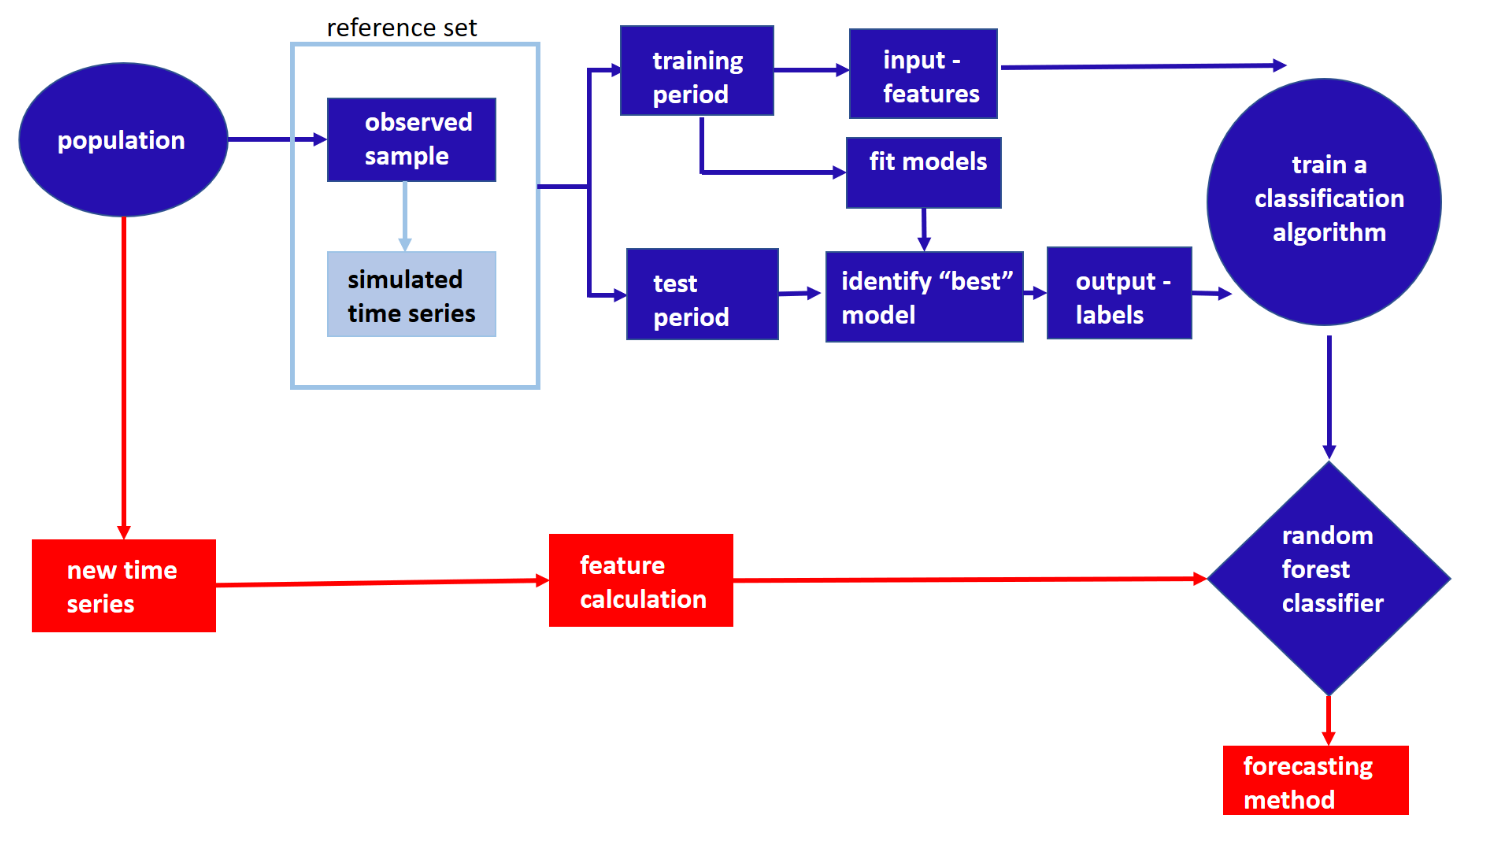
\includegraphics[width=\textwidth]{figures/FFORMS.png}
	\caption{Schematic diagram of the FFORMS framework. The offline phase is shown in red, the online/training phase is shown in blue.}
	\label{fig:FFORMS}
\end{figure}

\subsubsection{Meta-weighted Ensemble\cite{hyndman}}
Montero-Manso et al (2018) trained a gradient boosted tree model to learn the weights for a weighted ensemble of simple forecasting methods, and entered their model in the M4 forecasting competition. They used the M4 competition dataset. No augmentation was necessary. While training the model they performed a search over the hyper-parameter space of the gradient boosted tree model, using cross-validation to find the best hyper-parameters. They extracted forty-two features from each of the time series in training.

To use the model for any new time series, the features are extracted and the forecasts of the simple methods are calculated. The model then takes the time series and the features and outputs a vector of real numbers the same length as the number of forecasting methods. These numbers are transformed into probabilities using a softmax function.

The \textit{softmax} function is a squashing function which can take an arbitrary vector of real numbers $\mathbf{x} \in \mathbb{R}^n$ and transform it into a vector of values between $0$ and $1$ that sum to $1$. Formally,
\begin{align}
	\sigma : \mathbb{R}^n \rightarrow& \left\{ \sigma(\mathbf{x}) \in \mathbb{R}^n : \sigma(\mathbf{x})_j > 0 \forall j, \sum_{j=1}^n \sigma(\mathbf{x})_j = 1 \right\} \\
	\sigma(\mathbf{x})_i &= \frac{e^{\mathbf{x}_i}}{\sum_{j=1}^n e^{\mathbf{x}_j}}
\end{align} 
The softmax function is used in multi-class classification where a linear regression model is passed through a softmax function to give categorical probabilities. In this case there is one probability for each of the forecasting methods. These probabilities are used to combine the forecasts linearly in order to produce a single forecast.

In order to calculate prediction intervals, the model calculates the prediction intervals radius of a subset of the forecasting methods. A subset is taken for computational cost reasons. These radii are combined linearly using a weight matrix which is learned in training to give an upper and lower value for the interval for each time step in the forecasting horizon.

\section{Time Series Features}
\subsection{Spectral Entropy}
\subsubsection{Shannon's Entropy}
Shannon's Entropy aka. Information Entropy is a measure of the unpredictability of a random variable. If $X$ is a random variable with possbile values ${x_1, \dots, x_N}$ and associated probabilities $P(X=x_1), \dots, P(X=x_N)$, the entropy of the random variable $X$ is
\begin{align}
	H(X) 	&= -\sum_{n=1}^N P(X = x_n)\log P(X = x_n) \label{eq:entropy}\\
		&= \sum_{n=1}^N P(X = x_n) \log \frac{1}{P(X=x_n)}
\end{align}
The entropy of a continuous random variable is defined similary, but with integrals instead of summations.

If the variable is uniformly distributed across its values, then its entropy is maximised. If $X$ only ever takes one of its possible values, then $H(X)=0$. Usually the $\log$ in equation \ref{eq:entropy} is taken to the base $2$, and the entropy is therefore measured in \textit{bits}.

\subsubsection{Frequency Representation of Time Series}
Any time series can be expressed as a function of freqencies instead of as a function of time. The Fourier transformation transforms a time series into its frequency representation
\begin{align}
	x(f) = \int_{-\infty}^{\infty} e^{-2\pi i f t}x(t) dt
\end{align}
The \textit{power spectrum} of the time series is $S(f) = \modu{x(f)}^2$. The normalised power spectrum is
\begin{align}
	P(f) = \frac{S(f)}{\sum_{f^{\prime}}S(f^{\prime})}
\end{align}

The normalised power spectrum of a time series takes the form of a probability distribution and therefore defines a random variable over the frequencies $f^{\prime}$. The information entropy of this random variable is the \textit{spectral entropy} of the time series.

\subsection{Stability \& Lumpiness}
If a time series of length $L$ is divided up into non-overlapping windows of $\tau$ time-steps, and a variance is measured from the data within each window, then the \textit{stability} is the mean of the variances, and the \textit{lumpiness} is the variance of the variances. There are \texttt{R} functions for both of these quantities.

\section{Recurrent Neural Networks}
Recurrent neural networks (RNNs) are linear combinations of non-linear \textit{activation} functions applied to inputs combined in a way that is specifically designed for performing calculations on sequences, including time series.

In figure \ref{fig:forward_propagation} a schematic diagram of a simple recurrent neural network is shown. The $x$s are the inputs, for example a given time series. The $a$s are the activation values. The $y$s are the outputs. In this example network, the activations and outputs are defined by 
\begin{align}
	a^{\langle t \rangle} &= f(W_{aa}a^{\langle t-1 \rangle} + W_{ax}x^{\langle t \rangle} + b_a) \\
	&= f(W_{a}[a^{\langle t-1 \rangle}, x^{\langle t \rangle}] + b_a) \\
	y^{\langle t \rangle} &= g(W_{ya}a^{\langle t \rangle} + b_y)
\end{align}
where $f$ and $g$ are some non-linear \textit{activation functions}, such as $\tanh$, or the sigmoid function. There are a lot of possible variations to the network architecture. The output for step $t$ could be used as part of the input to step $t+1$ for example, or there could be connections that skip over one or more time steps, or outputs may not be produced until after all the inputs have been processed. The activation functions need not be just one function, there could be several functions connected to make up a smaller network which gives the activation function.

For choosing activation functions there are a lot of potential functions from which to choose. There are some characteristics that would be beneficial for an activation function.
\begin{description}
	\item[Non-linearity] It has been proven that a two layer neural network with non-linear activation functions can approximate any function. Also, to capture non-linear dynamics requires non-linear functions.
	\item[Continuously Differentiable] This makes gradient based optimisation easier. 
	\item[Monotonicity] If the activation function is monotonic, the error surface for a one-layer neural network is guaranteed to be convex. Meaning that there is only one optimum point, no local optima where an optimisation algorithm can get stuck.
	\item[Smooth (Infinitely Differentiable) functions with a Monotonic derivative] These have been shown to generalised better in some cases (apparently).
	\item[Approximates the identity function near the origin] If the activity function looks like the identity function $f(x) = x$ near the origin, then the network will learn efficiently when the paramters are initialised to small values. So this gives a good starting point for optimisation. If $f(0) = 0$, $f^{\prime}(0) = 1$, and $f^{\prime}$ is continuous around 0, then it's fair to say that $f$ approximates the identity around the origin.
\end{description}

The range or codomain of the function will have an effect on the network also. If the range of the function is restricted to some interval then gradient descent optimisation methods tend to be stable as the value of the gradient is very small for most values. On the other hand, the training process will suffer from the vanishing gradient problem causing learning to slow down as training goes on. $\tanh$ and the sigmoid function are examples of activation functions with ranges restricted to an interval. If the range of the function is unrestricted, training tends to be more efficient as the gradient of the activation function doesn't disappear, but a smaller learning rate may be necessary to find the optimum. The rectified linear unit and any other activation fuctions like that have unrestricted ranges. \footnote{A fairly comprehensive list of candidate activation functions can be found here: \url{https://en.wikipedia.org/wiki/Activation_function}}

\begin{figure}[ht]
	\centering
	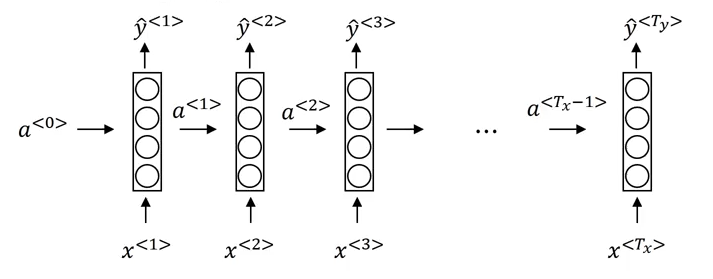
\includegraphics[width=\textwidth]{figures/forward_propagation.png}
	\caption{Schematic diagram of a simple recurrent neural network. The $x$s are inputs, the $a$s are the activations, and the $y$s are outputs.}
	\label{fig:forward_propagation}
\end{figure}

The backpropagation algorithm is used to train RNNs, just like any neural network. If the gradient of the loss function is propagated back through all of the time steps in the input sequence, the gradient may become exponentially small, or exponentially large. This is called the vanishing gradient problem, or exploding gradient problem, respectively. A vanishing gradient will make it difficult for information or errors (and error correction) to propagate along the RNN and will inhibit learning over time. An exploding gradient will make learning impossible as the gradient becomes too large to compute. 

The vanishing gradient problem is more common in RNNs, and the exploding gradient problem is easier to deal with. Therefore, many of the innovations in RNNs are attempts to solve the vanishing gradient problem. The most well known and widely used of these is the \textit{long-short term memory unit}, or LSTM (see section \ref{sec:lstm}). There have been some innovations on the LSTM idea. The Gated Recurrent Unit (GRU) and the Just Another Net (JANET) will be covered here. 

The LSTM, GRU, and JANET are examples of `cells' or `neurons' that can be stacked and connected in order to build the RNN. There have also been innovations in the way the RNNs are connected, i.e. the \textit{architecture} of the network.

\subsection{Cell Innovations: LSTM, GRU, JANET}

\subsubsection{Long-Short Term Memory Unit (LSTM)}\label{sec:lstm}
Each of the neurons in the RNN can take the form of an LTSM. So the LSTM will take an input $x^{\langle t \rangle}$ and an activation $a^{\langle t-1 \rangle}$ from the previous time step, and will output an activation. The activation could then be used to create an output for the RNN. The LSTM is defined by
\begin{align}
	\tilde{c}^{\langle t \rangle} &= \tanh(W_c[a^{\langle t-1 \rangle}, x^{\langle t \rangle}] + b_c) \label{eq:lstm_cand} \\
	\Gamma_u &= \sigma(W_u[a^{\langle t-1 \rangle}, x^{\langle t \rangle}] + b_u) \label{eq:lstm_update} \\
	\Gamma_f &= \sigma(W_f[a^{\langle t-1 \rangle}, x^{\langle t \rangle}] + b_f) \label{eq:lstm_forget} \\
	\Gamma_o &= \sigma(W_o[a^{\langle t-1 \rangle}, x^{\langle t \rangle}] + b_o) \label{eq:lstm_output} \\
	c^{\langle t \rangle} &= \Gamma_u \odot \tilde{c}^{\langle t \rangle} + \Gamma_f \odot c^{\langle t-1 \rangle} \label{eq:lstm_cell} \\
	a^{\langle t \rangle} &= \Gamma_o \odot \tanh( c^{\langle t \rangle}) \label{eq:lstm_act}
\end{align}
where $\odot$ represents element-wise multiplication and $\sigma$ represents the sigmoid function. The $c^{\langle t \rangle}$ quantity can be interpreted as an internal value for the LSTM. The LSTM is sometimes referred to as a `cell', so the letter `c' is used. The $\tilde{c}^{\langle t \rangle}$ quantity can be interpreted as a candidate for the updated internal value which is calculated using the current input $x^{\langle t \rangle}$ and the activation of the previous time-step $a^{\langle t-1 \rangle}$ in equation \ref{eq:lstm_cand}. Equations \ref{eq:lstm_update}, \ref{eq:lstm_forget}, and \ref{eq:lstm_output} are the \textit{update}, \textit{forget}, and \textit{output} gates respectively. The first two of these gates together with equation \ref{eq:lstm_cell} control the update to the internal value of the cell. The updated internal value $c^{\langle t \rangle}$ will be a combination of the candidate update and the previous internal value $c^{\langle t-1 \rangle}$. The activation of the unit $a^{\langle t \rangle}$ is a non-linear function of the updated internal value scaled by the output gate. A schematic diagram of an LSTM can be seen in figure \ref{fig:lstm}.

\begin{figure}[ht]
	\centering
	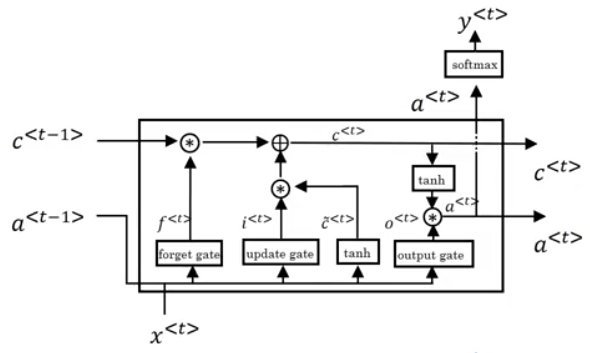
\includegraphics{figures/lstm.png}
	\caption{Schematic diagram of an LSTM.}
	\label{fig:lstm}
\end{figure}

The whole network of the LSTM and in particular equation \ref{eq:lstm_cell} allows for errors, and therefore gradients, to propagate back through the network without diminishing in size. Equation \ref{eq:lstm_cell} defines a state within the cell that may not be affected by incoming inputs and activations depending on the update and forget gates. Since the update and forget gates are defined using the sigmoid function, these gates must be between $0$ and $1$. Furthermore, the value of these gates is likely to be pushed towards 0 or 1 by the back propagation process. So, these gates can be intuitively interpreted as a vector of binary values of the same length as the input. Therefore the parameters $W_u$ and $W_f$ should allow the RNN to learn when the value of a certain input or activation will have an effect on an output much later on in the input time series. This is the `memory' referred to in the title of the LSTM.

\subsubsection{Gated Recurrent Unit (GRU)\cite{cho, chung}}
The GRU can be seen as a simplification of the LSTM because it avoids the vanishing gradient function in the same way as the LSTM, but using fewer equations and fewer parameters. Similar to the LSTM, the GRU uses an internal value or `state' which might be updated slightly or updated a lot at every time step. But the GRU uses this state as its activation, so there is no need for an output gate. The GRU also disregards the forget gate, and uses a single update gate to decide by how much the internal state will be updated. The only addition to the LSTM in the GRU is a \textit{relevance gate}, which is designed to capture the relevance of the previous state (combined with the input) to the candidate state.

\begin{align}
	\Gamma_r &= \sigma(W_r[c^{\langle t-1 \rangle}, x^{\langle t \rangle}] + b_r) \label{eq:gru_rel} \\
	\tilde{c}^{\langle t \rangle} &= \tanh(W_c[\Gamma_r \odot c^{\langle t \rangle},x^{\langle t \rangle}] + b_c) \label{eq:gru_cand} \\
	\Gamma_u &= \sigma(W_u[c^{\langle t-1 \rangle}, x^{\langle t \rangle}] + b_u) \label{eq:gru_update} \\
	c^{\langle t \rangle} &= \Gamma_u \odot \tilde{c}^{\langle t \rangle} + (1 - \Gamma_u) \odot c^{\langle t-1 \rangle} \label{eq:gru_cell}
\end{align}

Equation \ref{eq:gru_rel} is the relevance gate, mentioned above. Equation \ref{eq:gru_cand} defines the candidate state. Equation \ref{eq:gru_update} defines the update gate, similar to the LSTM. Equation \ref{eq:gru_cell} defines the the updated internal state. A schematic diagram of a GRU is shown in figure \ref{fig:gru}.

\begin{figure}[ht]
	\centering
	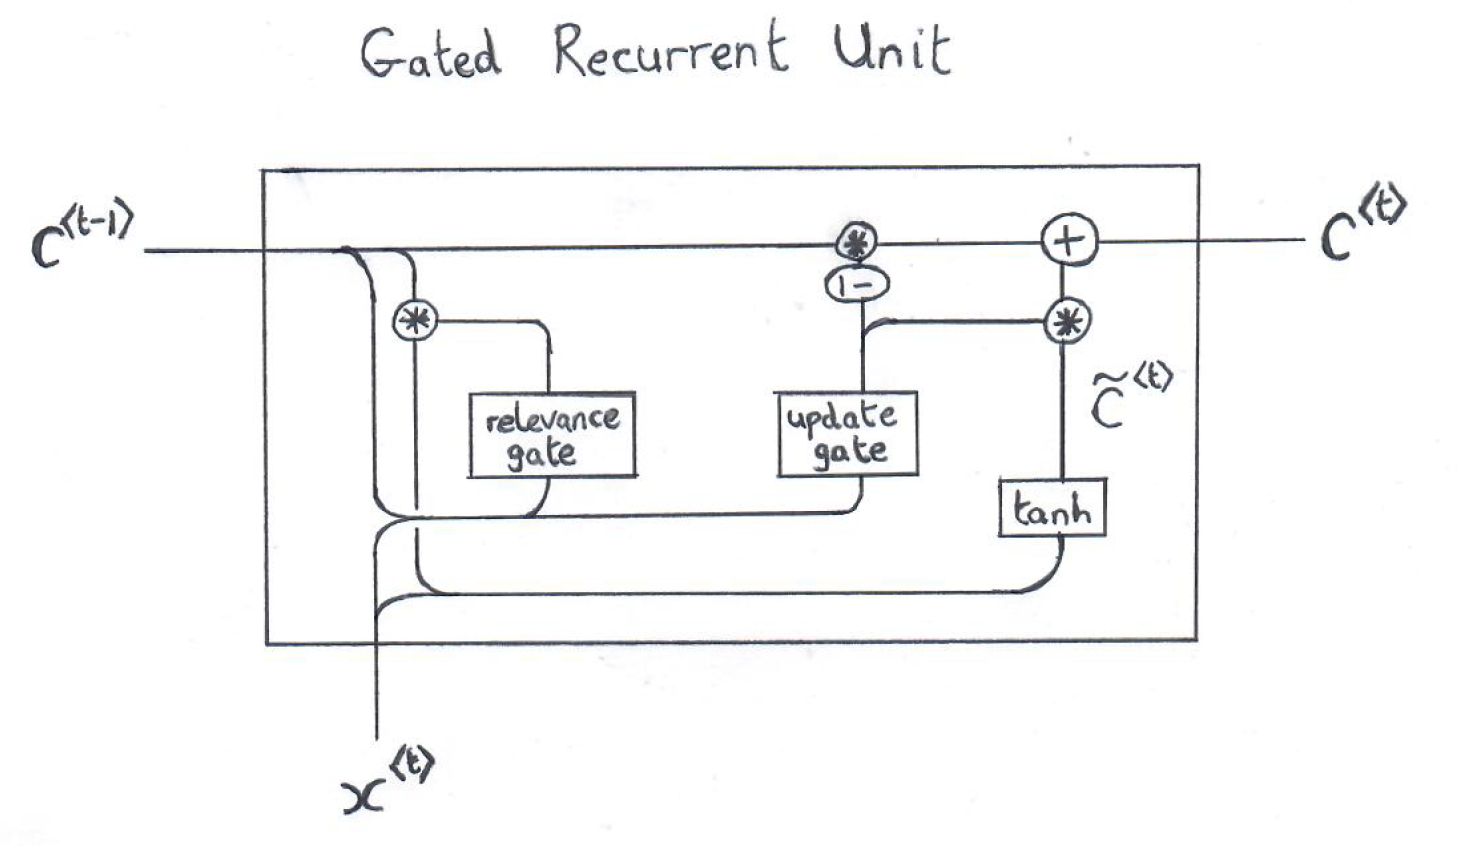
\includegraphics[width=\textwidth]{figures/gru.png}
	\caption{Schematic diagram of a GRU.}
	\label{fig:gru}
\end{figure}

GRUs have been found to be comparable to LSTMs in certain circumstances and to outperform LSTMs on smaller datasets \cite{chung}. 

\subsubsection{Just Another Net (JANET)\cite{janet}}
The JANET is another simplification of the standard LSTM. Van der Westhuizen et al (2018) removed the update and output gates from the LSTM, leaving only the forget gate. They also subtracted a constant from the argument for the forget gate when acting on the candidate state. The idea being that this would make it easier for information to accumulate in the cell's memory. The JANET is defined by
\begin{align}
	s^{\langle t \rangle} &= W_f[c^{\langle t-1 \rangle}, x^{\langle t \rangle}] + b_f \label{eq:janet_in} \\
	\tilde{c}^{\langle t \rangle} &= \tanh(W_c[c^{\langle t-1 \rangle}, x^{\langle t \rangle}] + b_c) \label{eq:janet_cand} \\
	c^{\langle t \rangle} &= \sigma(s^{\langle t \rangle}) \odot c^{\langle t-1 \rangle} + (1 - \sigma(s^{\langle t \rangle} - \beta)) \odot \tilde{c}^{\langle t \rangle} \label{eq:janet_cell}
\end{align}
Equation \ref{eq:janet_in} defines the \textit{input control component}. This would usually be the argument of the sigmoid function in the forget gate. But the forget gate takes a slightly different form here, so it is easier to define the cell this way. Equation \ref{eq:janet_cand} is the usual candidate definition. Equation \ref{eq:janet_cell} defines the updated internal state. The first term of this equation is standard and controls how much the remembered state contributes to the updated state. The second term is standard except for the subtraction of the $\beta$. This subtraction reduces the contribution of the candidate state to the updated state, which helps the JANET's `memory' accumulate. In \cite{janet}, the authors found that setting $\beta=1$ gave the best results on the tests performed. Similar to the GRU, the JANET uses the updated state $c^{\langle t \rangle}$ as its activation. A schematic diagram of a JANET is shown in figure \ref{fig:janet}.

\begin{figure}[ht]
	\centering
	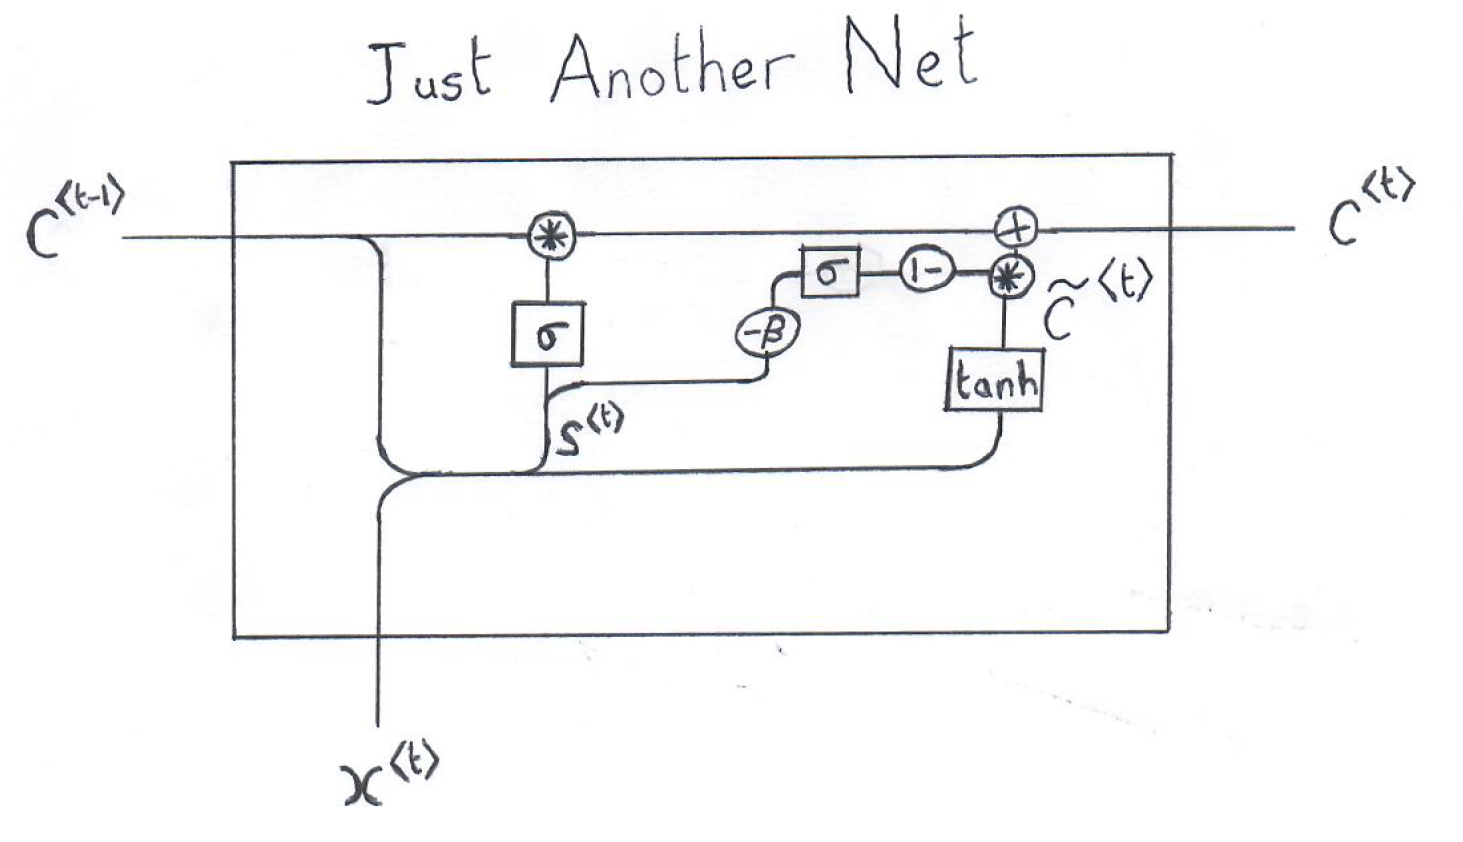
\includegraphics[width=\textwidth]{figures/janet.png}
	\caption{Schematic diagram of a JANET.}
	\label{fig:janet}
\end{figure}

The process of \textit{chrono initialization} detailed in \cite{tallec} was used to improve the JANET's performance. This amounts to initialising the bias of the forget gate $b_f$ to a \textit{characteristic forgetting time}, which is defined by the longest time dependency that the network will have to capture. This dependency is defined by the user when setting up the network.

Van der Westhuizen et al tested the JANET using some standard tests for RNNs such as testing the performance on the MNIST dataset, and the permuted MNIST dataset. They found that the JANET outperformed the standard LSTM on all the tests performed. A JANET was also used as part of the CFM competition to predict future volatility based on past volatility. The user reported better performance than a regualr LSTM, while using fewer parameters \cite{cfm}.

\textbf{N.B.:} The JANET was outperformed by something called the \textit{tensorised LSTM (tLSTM)} \cite{he}. May be worth looking into.

\subsection{Architectural Innovations}

\subsubsection{Dilated Recurrent Neural Networks \cite{chang}}
A skip connection in a recurrent neural network is an extra connection between two time steps a number of time steps apart. The normal connections in the RNN are still there. A dilated recurrent skip connection is a connection between steps in a recurrent neural network that skips one or more of the next steps without the normal one-step connections. A schematic diagram of a dilated skip connection can be seen in figure \ref{fig:dilated_connection} as compared to a standard skip connection. This has the effect of reducing the number of layers through which an error must be back propogated, which addresses the vanishing gradient problem, reduces the number of parameters in the network, and forces the network to learn some historical dependencies. The dilated skip connections also allow calculations to be performed in parallel, thereby exploiting the parallelising power of a GPU. 

\begin{figure}[ht]
	\centering
	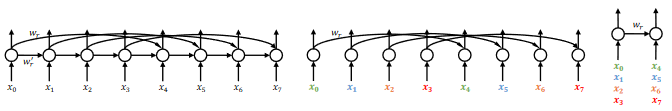
\includegraphics[width=\textwidth]{figures/dilated_skip_connection.png}
	\caption{(left) A one layer recurrent neural network with a skip connections. (middle) A one layer recurrent neural network with dilated recurrent skip connections. (right) A structure equivalent to the middle network. The input sequence length is reduced by four, and each of the four sequences can be processed in parallel.}
	\label{fig:dilated_connection}
\end{figure}

If the activation of a cell in layer $l$ and time $t$ of an RNN with standard skip connections is denoted by $c^{\langle t \rangle(l)}$, then 
\begin{align}
	a^{\langle t \rangle(l)} = f\left(x^{\langle t \rangle(l)}, a^{\langle t - 1 \rangle(l)}, a^{\langle t - s^{(l)} \rangle(l)}\right)
\end{align}
The activation of a similar cell in an RNN with dilated skip connections is
\begin{align}
	a^{\langle t \rangle(l)} = f\left(x^{\langle t \rangle(l)}, a^{\langle t - s^{(l)} \rangle(l)}\right)
\end{align}
where $s^{(l)}$ is the length of the skip connection in layer $l$, $x^{(l)}$ is the input to layer $l$, and $f$ is a function that could represent any linear or non-linear function or collection of functions commonly used in an RNN, including LSTM, GRU, etc.

A dilated recurrent neural network is one where dilated layers are stacked together in order to form a complete network. The dilation in each layer should increase exponentially. This makes different layers focus on different temporal resolutions, and reduces the average length of paths between nodes at different time points (proof in \cite{chang}). An example dilated RNN with three layers and a dilation of two can be seen in figure 

\begin{figure}[ht]
	\centering
	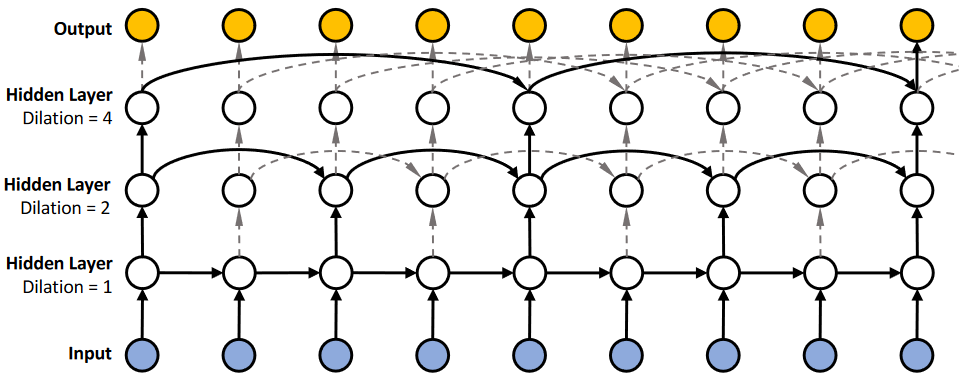
\includegraphics[width=\textwidth]{figures/dilated_rnn.png}
	\caption{An example of a dilated RNN with three layers with dilations of 1, 2, and 4, respectively.}
	\label{fig:dilated_rnn}
\end{figure}

The dilations in a dilated RNN can cause missing dependencies in the output layer. These dependencies can be reintroduced by including convolutional connections from the final hidden layer to the output layer.

In order to test the performance of the dilated RNN, Chang et al uses the \textit{copy memory problem}. This task tests the ability of recurrent models to memorise long-term information. Each input sequence is of length $T+ 20$. The first ten values are randomly generated from integers 0 to 7, the next $T-1$ values are all 8, the last 11 values are all 9. The first occurance of a 9 tells the model that it must reproduce the first 10 digits. The random guess yields an expected average cross entropy of $\ln(8) \approx 2.079$. The results of the copy memory problem can be seen in figure \ref{fig:copy_memory_problem}.

\begin{figure}[ht]
	\centering
	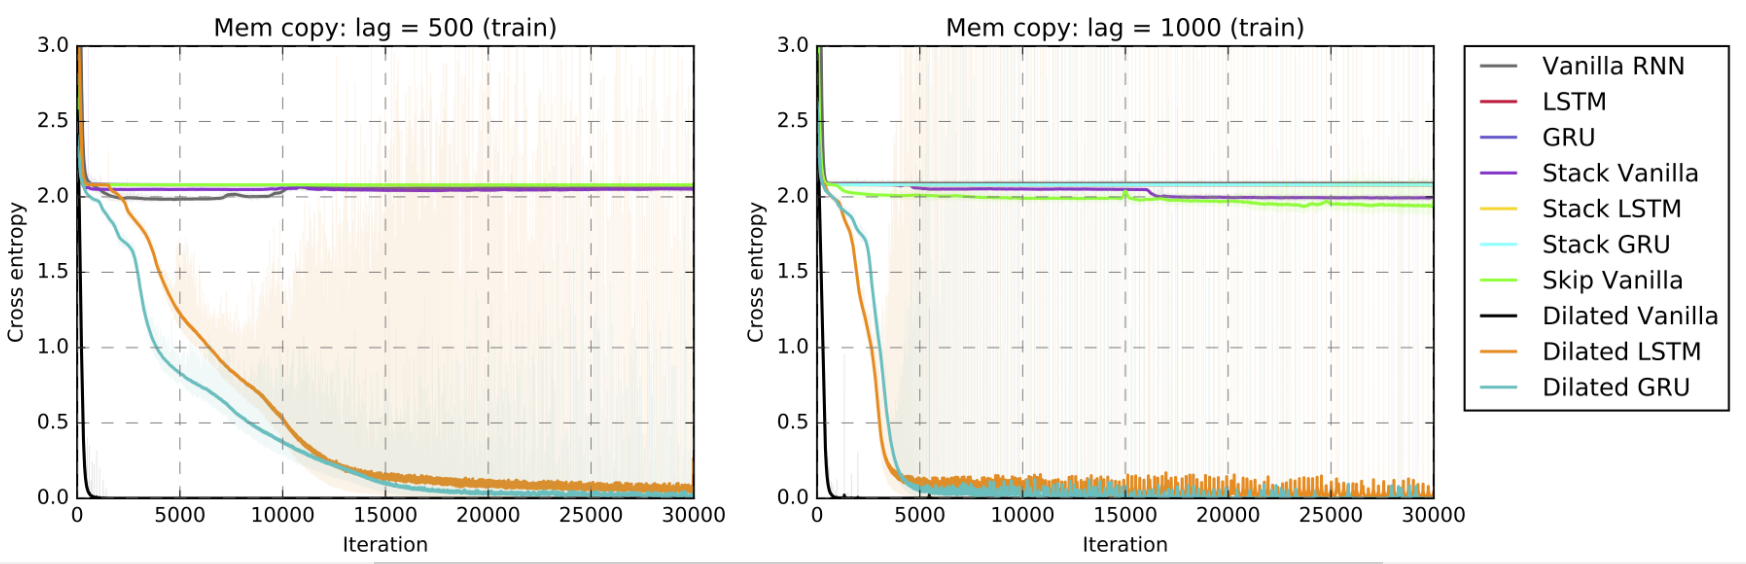
\includegraphics[width=\textwidth]{figures/copy_memory_problem.png}
	\caption{Results of the copy memory problem with $T= 500$ (left) and $T = 1000$ (right). Only RNNs with dilated skip connections converge to the perfect solution, all other methods are unable to improve over random guesses. }
	\label{fig:copy_memory_problem}
\end{figure}

Chang et al also used the MNIST dataset of handwritten digits to test the performance of various RNNs. The RNN was tasked with classifying the digit after reading in each of the pixels one-by-one as a $784 \times 1$ sequence. The results of the task can be seen in figure \ref{fig:dilated_mnist}. All the RNNs without skip connections failed at the task. The `Vanilla' RNN with standard skip connections showed some success. This is consistent with the finding that RNNs with skip connections are better at learning long term dependencies. The RNNs with dilated skip connections performed the best, with the dilated GRU showing the best performance after training.

\begin{figure}[ht]
	\centering
	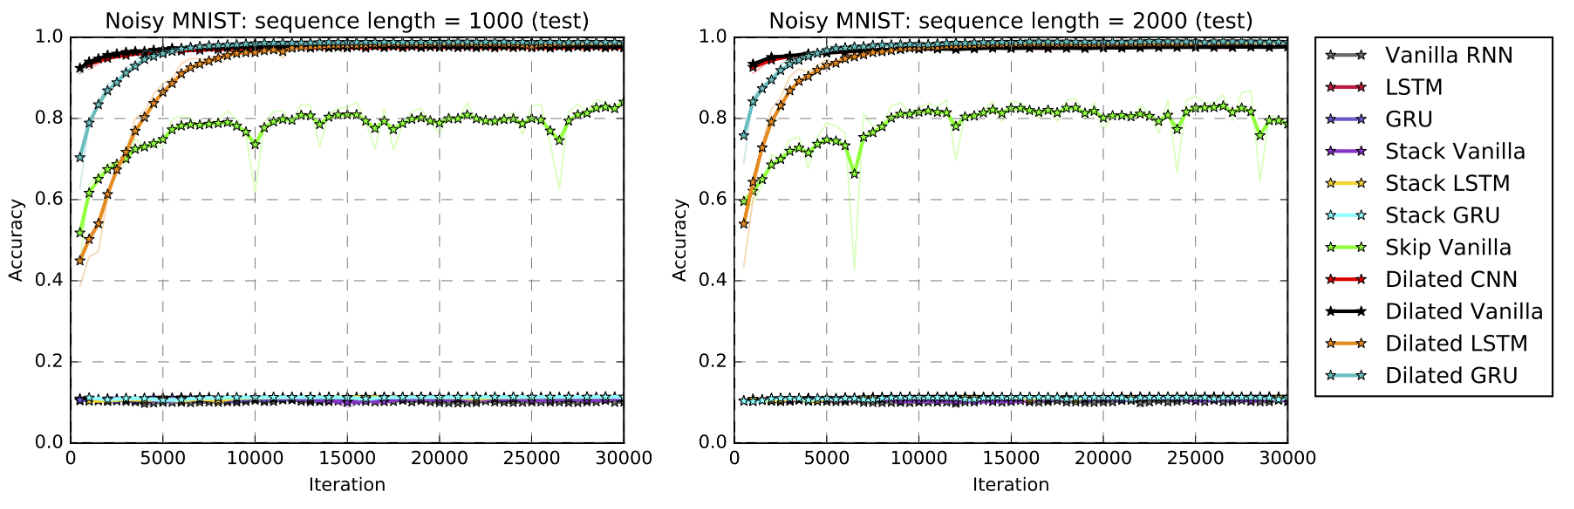
\includegraphics[width=\textwidth]{figures/dilated_mnist.png}
	\caption{Results of the MNIST classification task used by Chang et al to assess the performance of the dilated RNNs against other RNNs. The dilated RNNs perform the best, with the dilated GRU showing the best performance after training.}
	\label{fig:dilated_mnist}
\end{figure}

\subsubsection{The Attention Mechanism \cite{bahdanau}}
The attention mechanism deals with the case where there exists a target time series $y_1, \dots, y_{t-1} \in \mathbb{R}$ and $n$ driving (exogeneous) series $\mathbf{x}_1, \dots, \mathbf{x}_t \in \mathbb{R}^n$, and the objective is to learn a function $F$ such that $\hat{y}_t = F(y_1, \dots, y_{t-1}, \mathbf{x}_1, \dots, \mathbf{x}_t)$. 

The first step is encoding the driving series $(\mathbf{x}_1, \dots, \mathbf{x}_t) = \mathbf{X} \in \mathbb{R}^{n \times T}$. This is done using a bi-directional RNN. If $\mathbf{X}^{\top} \in \mathbb{R}^{T \times n}$ is a time series of vectors containing one element from each of the $n$ driving series, then a bi-directional RNN will read forward from $\mathbf{x}_1, \dots,\mathbf{x}_{T_x}$ calculating foward hidden states $\overrightarrow{h}_1, \dots, \overrightarrow{h}_{T_x}$, then read backward from $\mathbf{x}_{T_x}, \dots,\mathbf{x}_1$ calculating backward hidden states $\overleftarrow{h}_{T_x}, \dots, \overleftarrow{h}_1$. Concatenating these forward and backward hidden states together gives an encoding, also known as an annotation, $h_{t}$ which contains information from the whole time series of vectors, but is focussed around timestep $t$. It is common to use LSTMs or GRUs for these encoders. 

\begin{figure}[ht]
	\centering
	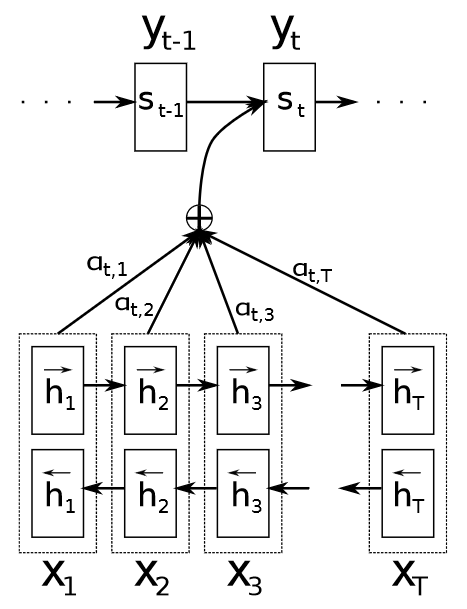
\includegraphics[width=0.5\textwidth]{figures/attention_mechanism.png}
	\caption{A schematic diagram of an RNN with an attention mechanism. The inputs $\mathbf{X}_t$ are encoded by a bi-directional RNN into hidden states $h_t$. Those hidden states are combined with the decoder RNN hidden state $s_t$ in the attention model to create a context vector. The context vector is combined with the previous output, and the previous hidden state to create the next output.}
	\label{fig:attention_mechanism}
\end{figure}

The output of the network will come from a forward reading RNN, that reads in the last output $y_{t-1}$, the current hidden state $s_t$, and the current \textit{context vector} $c_t$. To calculate the context vector, the last hidden state of the output RNN is combined with the encoder hidden state corresponding to the current timestep $h_{t^{\prime}}$ in an \textit{alignment model},
\begin{align}
	e_{tt^{\prime}} = a(s_{t-1}, h_{t^{\prime}})
\end{align}
In \cite{bahdanau}, the alignment model $a$ takes the form of a feed-forward neural network that is trained along with the rest of the network. The $e_{tt^{\prime}}$ are combined to create attention coefficients, or attention weightings using the softmax function
\begin{align}
	\alpha_{tt^{\prime}} = \frac{\exp(e_{tt^{\prime}})}{\sum_{v=1}^{T_x} \exp(e_{tv})}
\end{align}
In the machine translation context $\alpha_{tt^{\prime}}$ is a probability that the target word $y_t$ is aligned to, or translated from, a source word $x_{t^{\prime}}$. These attention weightings are used to combine the hidden states linearly to make the context vector,
\begin{align}
	c_t = \sum_{v=1}^{T_x}\alpha_{tv}h_v
\end{align}
The context vector, the previous hidden state, and the previous output is combined to create the current hidden state of the output RNN
\begin{align}
	s_t = f(s_{t-1}, y_{t-1}, c_t)
\end{align}
and this hidden state is combined with the previous output and the context vector to create the conditional probability of the next output
\begin{align}
	P(y_t | y_{1},\dots,t_{t-1}, \mathbf{X}) = g(y_{t-1}, s_t, c_t)
\end{align}
The next output $y_t$ is sampled from this distribution. A schematic diagram of the attention mechanism, aka the attention model is shown in figure \ref{fig:attention_mechanism}.

The point here is to encode the amount of attention that should be paid to input $\mathbf{x}_{t^{\prime}}$ when calculating output $y_t$. This information is held in the attention weightings $\alpha_{tt^{\prime}}$ where $t,t^{\prime} \in {1, \dots, T}$. The attention weightings can be displayed as a kind of cross correlation matrix in order to discover where dependencies lie. The encoder-decoder architecture also allows the output length to vary regardless of the input length.

In \cite{bahdanau}, Bahdanau et al tested an RNN encoder-decoder with attention mechanism on English to French translation. A corpus of 348 million words was used. The BLEU score was used to asses the quality of the translation. The BLEU score assesses how well machine translation matches human translation, the closer the match, the higher the score. \footnote{For more information on the BLEU score see: \url{https://en.wikipedia.org/wiki/BLEU}} The RNN encoder-decoder with the attention mechanism (referred to as RNN-search) performance was compared to the performance of an RNN encoder-decoder without the attention mechanism (referred to as RNN-enc). Each type of model was trained using sentences of length up to 30 words, and then sentences of length up to 50 words. The results of the translation task are shown in figure \ref{fig:attention_results}. The network with the attention mechanism significantly outperformed the network without. Even the attention network trained with sentences up to 30 words in length outperformed the attention-less network trained with sentences up to 50 words in length when translating sentences  up to 60 words in length.

\begin{figure}[ht]
	\centering
	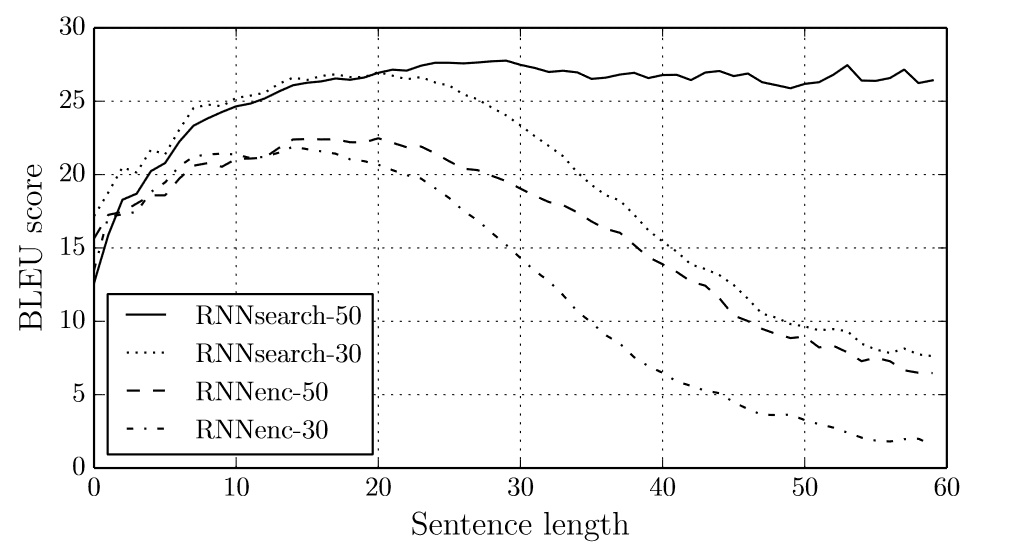
\includegraphics[width=\textwidth]{figures/attention_results.png}
	\caption{The RNN encoder-decoder with attention (RNN-search) and the RNN encoder-decoder without attention (RNN-enc) were used to translate English into French, and then assessed using the BLEU score system. Each type of model was trained with sentences up to 30 words in length, then up to 50 words in length. The RNN with the attention mechanism significantly outperformed the RNN without the attention mechanism, particularly the 50 word model on longer sentences.}
	\label{fig:attention_results}
\end{figure}


\subsubsection{Residual Network \cite{resnet}}
A residual network learns a function for the difference between the inputs and the outputs rather than a function to express the outputs given the inputs. Instead of learning the function $F$,
\begin{align}
	\mathbf{y} = F(\mathbf{x})
\end{align}
the residual network learns the function $H$
\begin{align}
	\mathbf{y} = H(\mathbf{x}) - \mathbf{x}
\end{align}
 The residual network is motivated by the \textit{degradation problem}, where an increase in the number of layers results in a disimprovement in both training and test error. Theoretically, if the added layers just learn the identity function there should be no degradation. This shows that some systems are more diffcult to optimise than others. The idea of the residual network is that it might be easier to optimise a network that learns residual functions instead of the usual output functions.

\begin{figure}[ht]
	\centering
	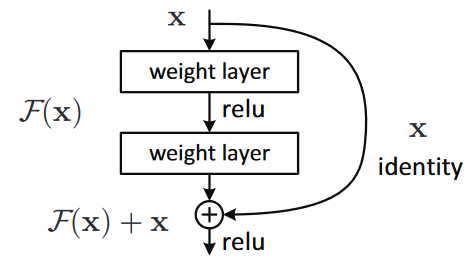
\includegraphics[width=0.5\textwidth]{figures/residual_rnn.png}
	\caption{A building block for a residual network. The input for the top layer is projected to the bottom layer, so the block learns a function for the difference between the input and output, i.e. the residual.}
	\label{fig:residual_rnn}
\end{figure}

In a residual network, the inputs for some given layer are fed back into the network two or three layers down. A block of a residual network can be seen in figure \ref{fig:residual_rnn}. A residual network was used to perform classification on the ImageNet database, and the inclusaion of the residual innovation on top of all the other tricks resulted in a classification error lower than human error \cite{resnet}. An example 34 layer neural network used on the ImageNet database, with and without residual connections is shown in figure \ref{fig:resnet}.
\begin{figure}[p]
	\centering
	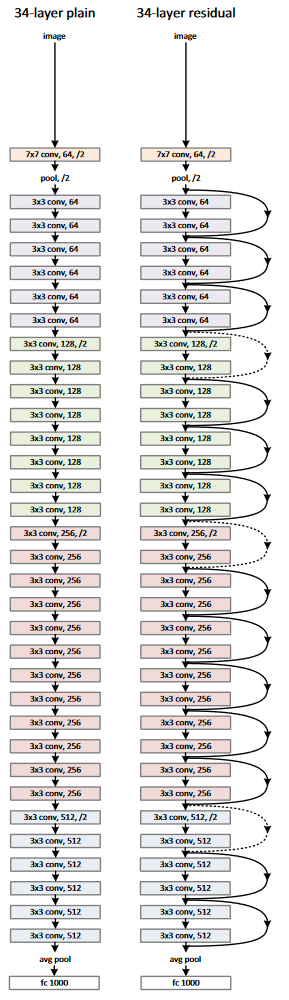
\includegraphics[width=0.42\textwidth]{figures/resnet.png}
	\caption{(left) A network architecture with 34 layers that was applied to the ImageNet database. (right) The same architecture with residual connections, making it a residual network.}
	\label{fig:resnet}
\end{figure}

\subsubsection{Residual LSTM \cite{kim}}
A residual LSTM is a standard LSTM with a residual innovation where the output of an LSTM in a higher layer is passed in additively before the output gate is applied. Equations \ref{eq:lstm_cand}, \ref{eq:lstm_update}, \ref{eq:lstm_forget}, \ref{eq:lstm_output}, and \ref{eq:lstm_cell} are all the same. A \textit{projection output} is defined by
\begin{align}
	m^{\langle t \rangle (l)} = W_m \tanh(c^{\langle t \rangle (l)})
\end{align}
the output from the previous layer's LSTM is added to this projection, then the output gate is applied
\begin{align}
	a^{\langle t \rangle (l)} = \Gamma_o \odot \left(m^{\langle t \rangle (l)} + W_{a^{\prime}}a^{\langle t \rangle (l-1)} \right) = \Gamma_o \odot \left(m^{\langle t \rangle (l)} + W_{a^{\prime}}x^{\langle t \rangle (l)} \right)
\end{align}
Essentially, the input to the LSTM is carried forward and reinserted just before last step of the LSTM processing. Each LSTM unit is a residual building block, similar but more complicated to that shown in figure \ref{fig:residual_rnn}.

in \cite{kim}, Kim et al used the AMI meeting corpus to evaluate residual LSTMs compared to standard LSTMs and highway LSTMs (LSTMs with a parametrised spacial skip connection). The AMI meeting corpus is a dataset of recordings of people meeting up and speaking English. The RNNs were trained to predict the next word for each speaker speaking at any given time. Both 3-layer and 10-layer networks were trained. The results of the AMI assessment for highway and residual LSTMs are shown in figure \ref{fig:lstm_AMI}. Both the training and cross-validation error for the 10-layer highway LSTM network are higher than that for the 3-layer. This indicates that the highway LSTM suffers from degredation. For the residual LSTM, although the training error is higher for the 10-layer network, the cross-validation error is lower for the deeper network. So the residual LTSM does not suffer from degredation. The higher training error for the deeper network could be due to better generalisation for data outside of the training set.

\begin{figure}
	\centering
	\begin{subfigure}[b]{0.49\textwidth}
		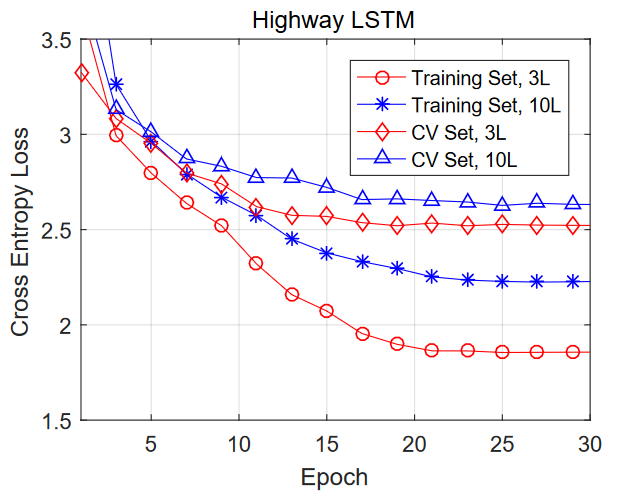
\includegraphics[width=\textwidth]{figures/highway_lstm_AMI.png}
		\caption{}
		\label{fig:highway_lstm_AMI}
	\end{subfigure}
	\begin{subfigure}[b]{0.49\textwidth}
		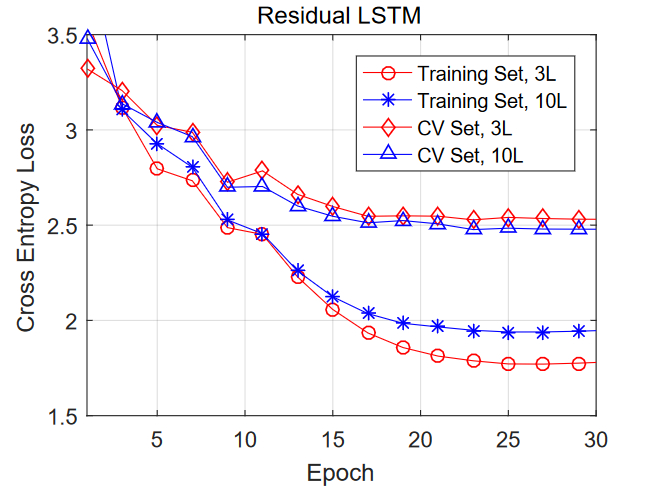
\includegraphics[width=\textwidth]{figures/residual_lstm_AMI.png}
		\caption{}
		\label{fig:residual_lstm_AMI}
	\end{subfigure}
	\caption{(a) The results of the AMI assessment on the highway LSTM network. Note that for both training and cross-validation, the cross-entropy error is higher for the deeper network. (b) The results of the AMI assessment on the residual LSTM network. Although the training error is higher for the deeper network, the cross validation error is lower for the deeper network.}
	\label{fig:lstm_AMI}
\end{figure}

The \textit{word error rate} (WER) for overlapping and non-overlapping speech was also assessed for standard LSTMs, highway LSTMs, and residual LSTMs. 3-layer, 5-layer, and 10-layer versions of each network were used. The results are shown in figure \ref{fig:wer}. Both the standard and highway LSTM networks have higher word error rates in general than the residual LSTM, and increasing word error rates for deeper networks. The residual LSTM network shows improving performance for deeper networks for non-overlapping speech.

\begin{figure}
	\centering
	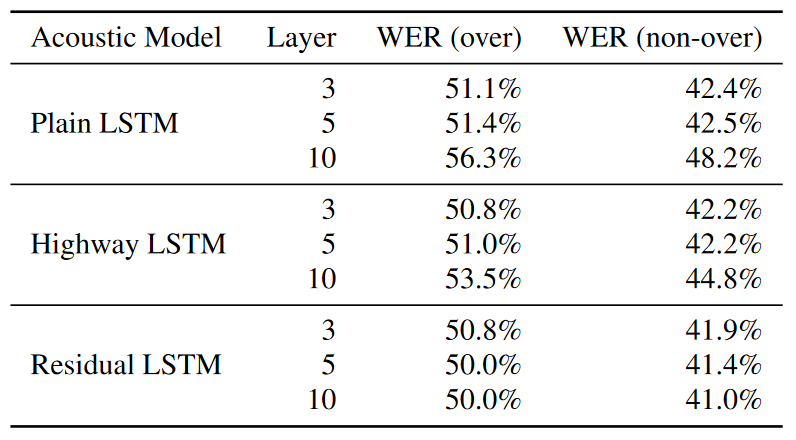
\includegraphics[width=0.75\textwidth]{figures/wer.png}
	\caption{Word error rates for overlapped and non-overlapped speech for standard LSTMs, highway LSTMS, and residual LSTMs, of depth 3, 5, or 10.}
	\label{fig:wer}
\end{figure}

\subsection{Example: Exponential Smooting RNN - M4 Competition Winner \cite{smyl}}
The winner of the M4 competition, a competition for time series forecasting, is a hybrid model combining exponential smoothing and RNNs. The model was implemented using DyNet and \texttt{C++}.

\subsubsection{Holt-Winter's Decomposition Preprocessing}
RNNs require a large amount of data in order to be trained. This usually means that they are trained with time series from different contexts. As a result of this, RNN models tend to over-generalise and their forecasts are not time-series specific. One particular problem is that RNN models struggle with seasonality. Smyl et al (2018) deal with this problem by using an Holt-Winter's seasonal model decomposition (see section \ref{sec:hw_seasonal}) as a preprocessing step. For each time series in the M4 dataset, the level and seasonality are calculated as
\begin{align}
	\ell_{t} &= \alpha \frac{y_t}{s_t} + (1 - \alpha)\ell_{t-1} \\
	s_{t+m} &= \gamma\frac{y_t}{l_t} + (1 - \gamma)s_t
\end{align}
then the forecasting equation is
\begin{align}
	\hat{y}_{t+1, \dots, t+h} = RNN(X_t)\odot \ell_t \odot s_{t+1, \dots, t+h}
\end{align}
where $X_t$ is a vector of a normalised and deseasonlised time series features, usually the length of one season, and includes the origin of the series in a binary vector the length of the number of categories.

Bear in mind that the parameters for the Holt-Winter's decomposition $\alpha$, $\gamma$, are learned for each time series separately. The parameters in the RNN are learned for all of the time series together. Therefore the mode is hierarchical in nature, part of the model deals with the time series individually, and part of the model deals with all of the dataset as one.

\subsubsection{RNN Architectures}
Three different RNN architectures were used to model yearly, quarterly, and monthly time series. A schematic diagram of the RNN for yearly data is shown in figure \ref{fig:uber_yearly}. The network consists of two layers of LSTM units using the attention mechanism and dilations, followed by a fully connected (aka dense) layer with a $\tanh$ activation function, followed by a linear adaptor layer. The linear adaptor layer transforms the output of the non-linear layer into the shape of the forecast horizon and produces upper and lower prediction intervals.

\begin{figure}[ht]
	\centering
	\begin{subfigure}[b]{0.32\textwidth}
		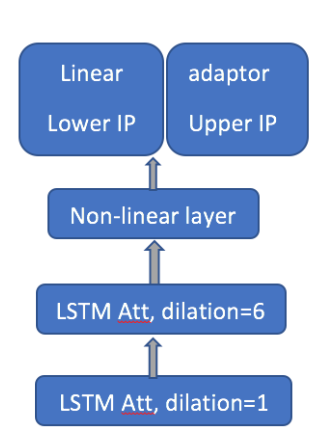
\includegraphics[width=\textwidth]{figures/uber_yearly.png}
		\caption{}
		\label{fig:uber_yearly}
	\end{subfigure}
	\begin{subfigure}[b]{0.32\textwidth}
		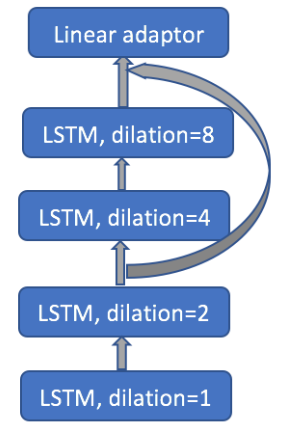
\includegraphics[width=\textwidth]{figures/uber_quarterly.png}
		\caption{}
		\label{fig:uber_quarterly}
	\end{subfigure}
	\begin{subfigure}[b]{0.32\textwidth}
		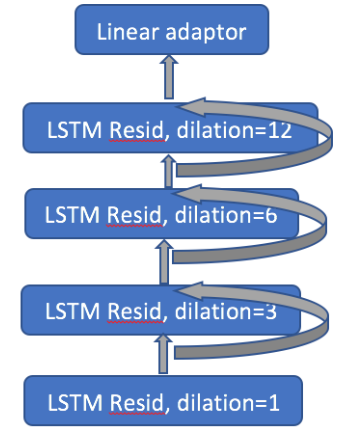
\includegraphics[width=\textwidth]{figures/uber_monthly.png}
		\caption{}
		\label{fig:uber_monthly}
	\end{subfigure}
	\caption{(a) A schematic diagram of the RNN architecture used by Smyl et al (2018) for forecasting \textbf{yearly} time series. (b) A schematic diagram of the RNN architecture used by Smyl et al (2018) for forecasting \textbf{quarterly} time series. (c) A schematic diagram of the RNN architecture used by Smyl et al (2018) for forecasting \textbf{monthly} time series.}
\end{figure}

A schematic diagram of the RNN used for quarterly data is shown in figure \ref{fig:uber_quarterly}. The network consists of four layers of LSTM units with exponentially increasing dilations. The top two layers of  LSTMs make up a `classical' residual block. The output layer is a linear adaptor that converts the size of the LSTM output to the size of the forecast horizon.

A schematic diagram of the RNN used for the monthly data is shown in figure \ref{fig:uber_monthly}. The network consists of four layers of residual LTSM units. Note that these are residual LSTMs, not residual connections around standard LSTMs. The output layer is a linear adaptor similar to that in the RNN for quarterly data.

\subsubsection{Loss Function}
The ES-RNN model uses a \textit{Pinball loss function}. 

A Pinball loss function is a loss function that measures the difference between the actual and forecasted values and introduces some bias to penalise positive errors more than negative errors, or negative errors more than positive errors. A Pinball loss function takes the form of 
\begin{align}
	L_Q(y_t - \hat{y}_t) =  	\begin{cases}
						Q(y_t - \hat{y}_t) &\quad \text{if } y_t \geq \hat{y}_t \\
						(Q-1)(y_t - \hat{y}_t) &\quad \text{if } y_t < \hat{y}_t
					\end{cases}
\end{align}
where $0 \leq Q \leq 1$. If $Q = 0.5$ then $L_Q(y_t - \hat{y}_t)$ is equivalent to the $\ell_1$ loss function. If $Q > 0.5$ then errors where $y_t \geq \hat{y}_t$ will be penalised more heavily than errors where $y_t \leq \hat{y}_t$.

For the ES-RNN model, $Q = 0.48$. This value was chosen to counteract positive bias that the authors noticed while developing the model.

For assessing the quality of prediction intervals, the M4 competition used the \textit{Mean Scaled Interval Score}, or MSIS,
\begin{align}
	MSIS(U_t, L_t, Y_t, h, a) = \frac{1}{h}\frac{\sum_{t=1}^h (U_t - L_t) + \frac{2}{a}(L_t - Y_t)\mathbf{1}\{ Y_t < L_t \} + \frac{2}{a}(Y_t - U_t)\mathbf{1}\{ Y_t > U_t \}}{\frac{1}{n-m}\sum_{t=m+1}^n\modu{Y_t - Y_{t-m}}}
\end{align}
where $U_t$ is the estimate for the upper prediction interval, $L_t$ is the estimate for the lower prediction interval, $h$ is the horizon, $a$ is a significance level ,and 
\begin{align}
	\mathbf{1}\{ \text{\textbf{conditional}} \} = 	\begin{cases}
									1 &\quad \text{ if \textbf{conditional} is true} \\
									0 &\quad \text{ if \textbf{conditional} is false} \\
								\end{cases}
\end{align}
is called the \textit{indicator function}. The ES-RNN model used the numerator of the MSIS function to train the model when forecasting prediction intervals.

\newpage

\bibliography{forecasting_lit_review.bbl}

\end{document}